\section{Evaluation}
\label{sec:evaluation}

\subsection{Experimental Setup}
\label{subsec:setup}

All experiments serve Llama-3.1-8B-Instruct~\cite{dubey2024llama3} in FP16
through vLLM on a single NVIDIA A100 GPU (40GB). Each scheduling policy is
evaluated at seven request arrival rates (5, 10, 20, 30, 40, 50, and 60
requests/second) on each dataset, with requests drawn in a fixed,
pre-computed admission order per policy and submitted to vLLM's offline
\texttt{LLM.generate()} API as a single call, so vLLM's own
continuous-batching scheduler manages iteration-level admission from that
point onward.

\subsection{Datasets}
\label{subsec:datasets}

We use two 1{,}000-request evaluation subsets constructed from the public
LMSYS-Chat-1M conversation dataset~\cite{zheng2023lmsyschat}. Dataset~1 is a
uniform in-distribution sample used to measure baseline scheduling behavior.
Dataset~2 over-samples the extremes of the true output-length distribution to
induce distribution shift between the predictor's training data and its
evaluation data, matching the out-of-distribution stress test used for the
original LTR predictor~\cite{fu2024efficient}. Both subsets are reconstructed
from the public dataset release rather than the original framework's
unpublished 23{,}800-sample file, and should be read as a reconstructed split
rather than an exact reproduction.

\subsection{Scheduling Policies and Metrics}
\label{subsec:policies-metrics}

The four scheduling policies compared are summarized in
Table~\ref{tab:scheduling_policies}. We report: (i) mean throughput in
tokens/second; (ii) two HOL blocking indicators, the ratio of p90 to mean
per-token latency at high load and the slope of mean latency against request
rate, where flatter and lower is better; (iii) time-to-first-token (TTFT),
the delay between arrival and the first generated token, computed from
vLLM's own per-request timestamps rather than approximated from aggregate
batch timing; (iv) peak GPU memory allocation and utilization; and (v)
Kendall's tau~\cite{kendall1938new} between each score and true output
length.

\subsection{Throughput}
\label{subsec:results-throughput}

Table~\ref{tab:throughput} reports mean throughput for each scheduler.
LTR + Prompt Length achieves the highest throughput of the four policies on
both datasets, improving over the original LTR scheduler by approximately
31.7\% on Dataset~1 and 6.7\% on Dataset~2. Notably, the original LTR and
Classification schedulers both under-perform plain FCFS on Dataset~1 despite
their explicit goal of reducing HOL blocking, suggesting that a miscalibrated
or overly aggressive reordering can trade away throughput even as it changes
tail-latency behavior; the composite score's use of prompt length as a
stabilizing signal appears to avoid this failure mode on the datasets tested.

\begin{figure*}[t]
    \centering
    \begin{subfigure}[b]{0.48\textwidth}
        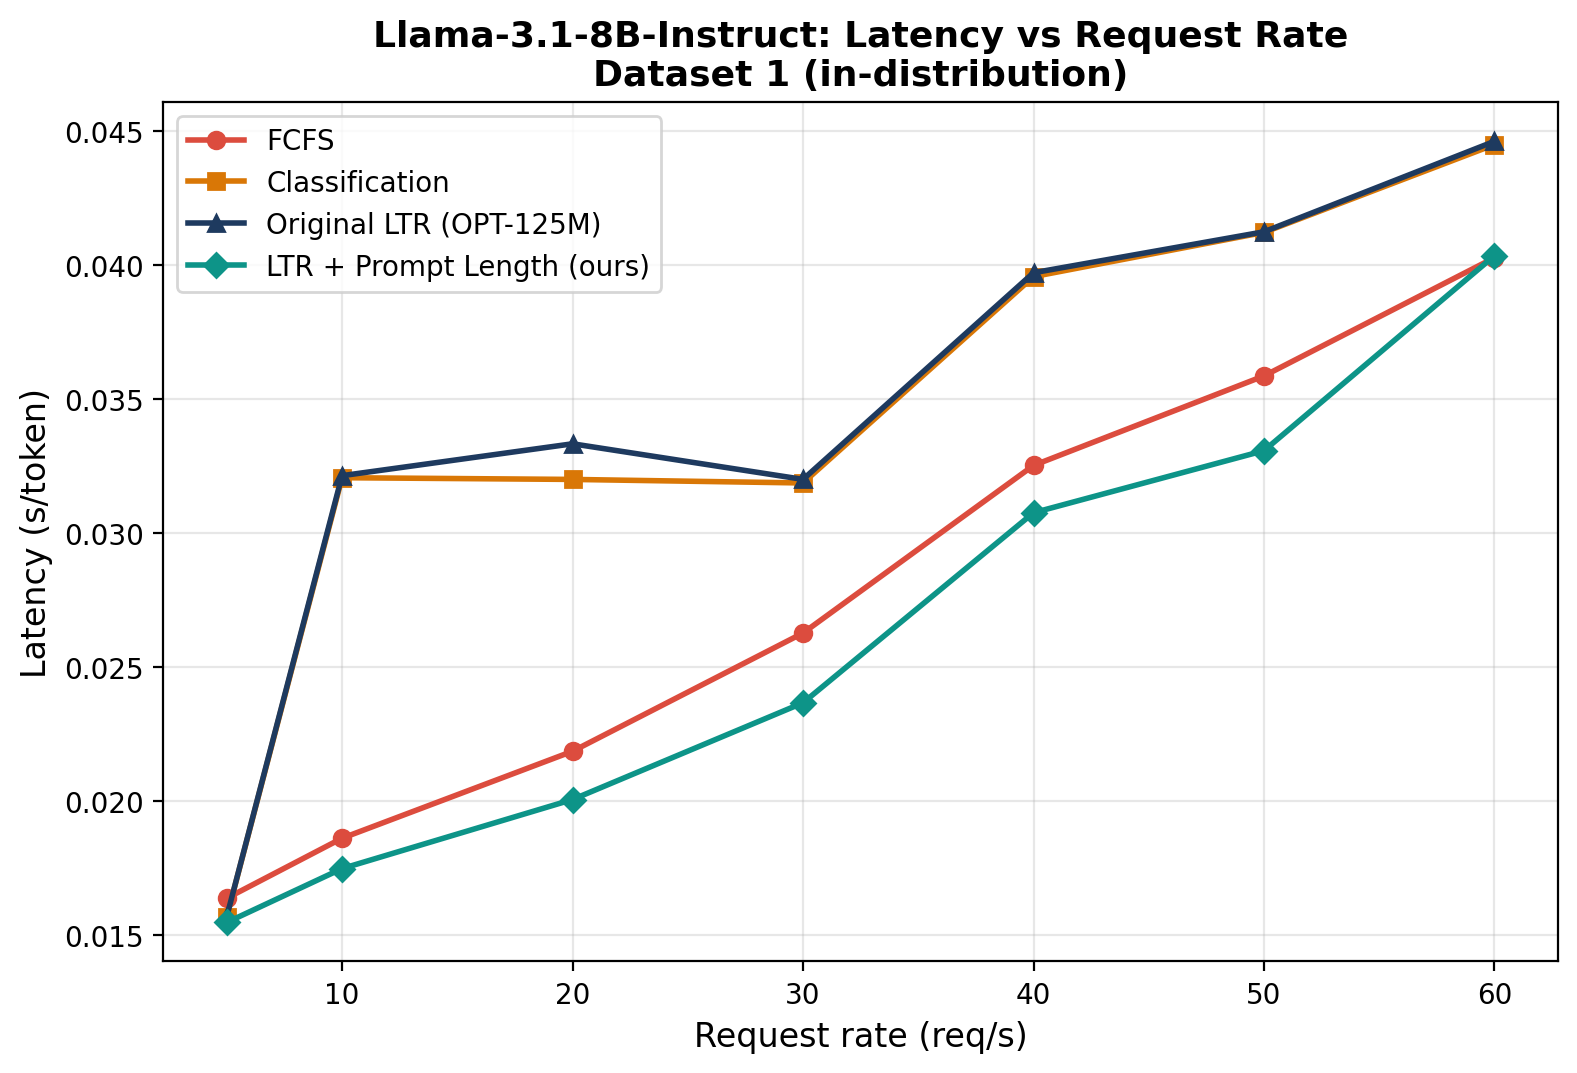
\includegraphics[width=\linewidth,height=3.5cm,keepaspectratio]{figures/latency_dataset1.png}
        \caption{Dataset 1 (in-distribution)}
        \label{fig:latency-d1}
    \end{subfigure}
    \hfill
    \begin{subfigure}[b]{0.48\textwidth}
        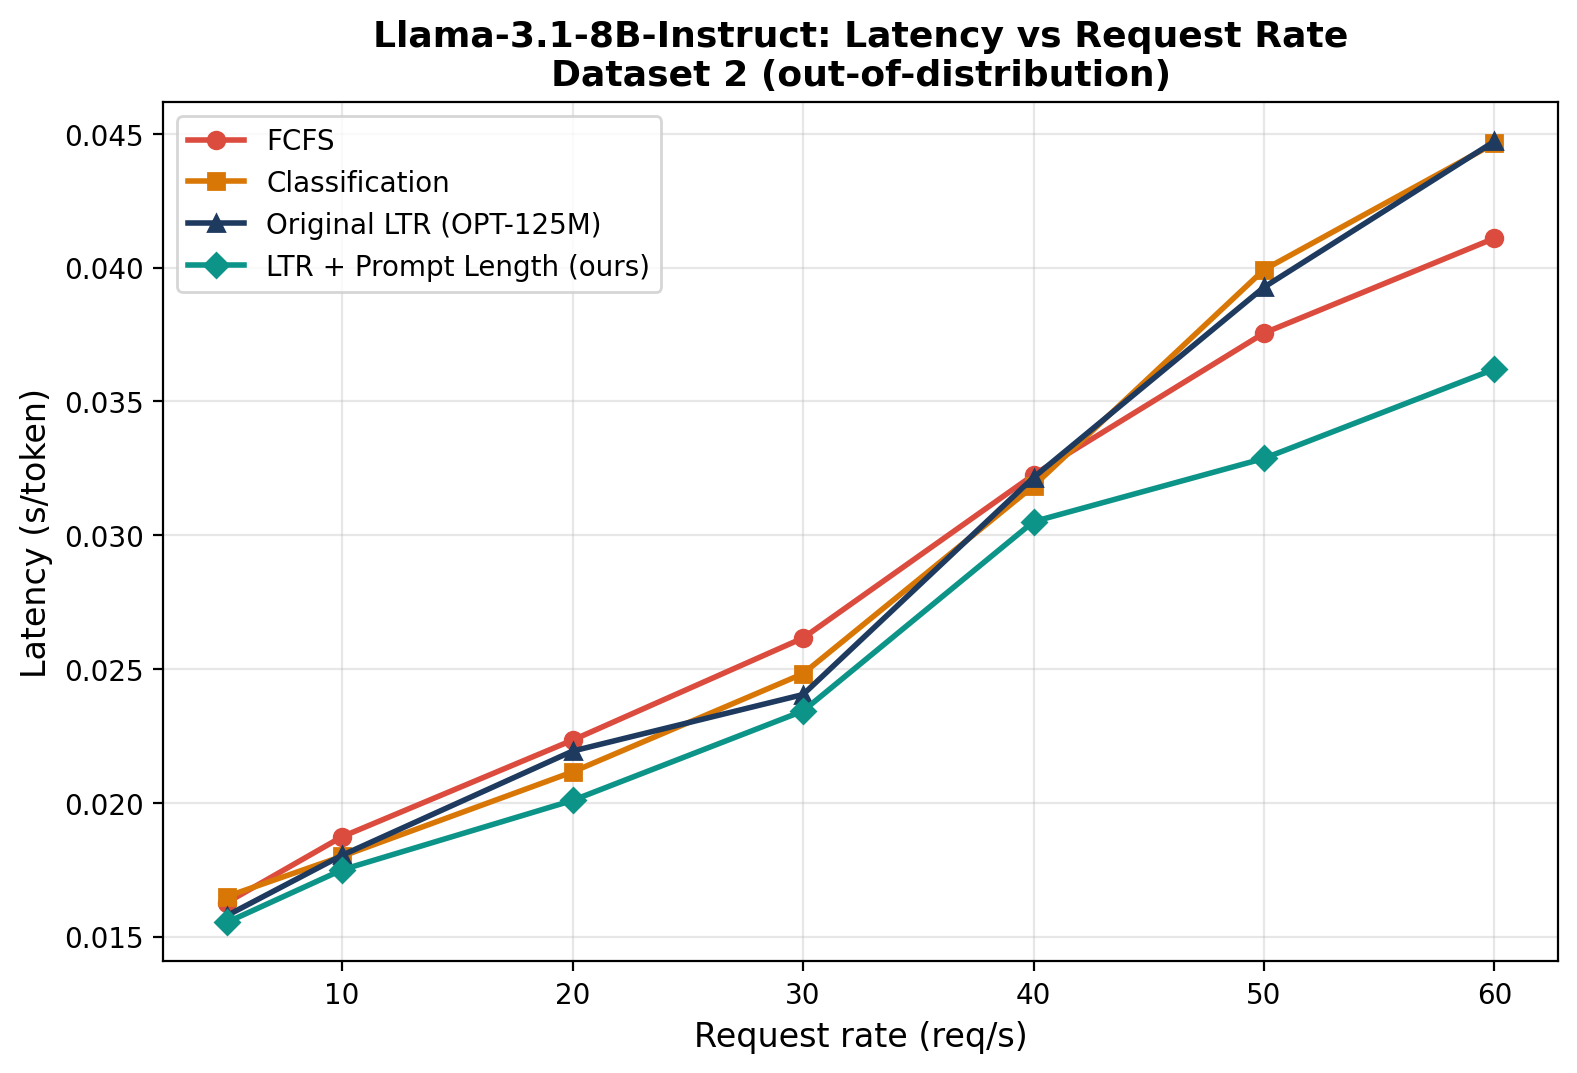
\includegraphics[width=\linewidth,height=3.5cm,keepaspectratio]{figures/latency_dataset2.png}
        \caption{Dataset 2 (out-of-distribution)}
        \label{fig:latency-d2}
    \end{subfigure}
    \caption{Mean per-token latency versus request rate, by scheduler.}
    \label{fig:latency-vs-rate}
\end{figure*}

\subsection{Latency Versus Request Rate}
\label{subsec:results-latency}

Figure~\ref{fig:latency-vs-rate} shows mean per-token latency as request rate
increases from 5 to 60 requests/second. All four policies show latency
rising with request rate, as expected once arrival rate approaches the GPU's
sustainable throughput, but the rate of increase differs by policy;
Table~\ref{tab:hol_blocking} quantifies this as the latency-vs-rate slope,
discussed in Section~\ref{subsec:results-hol}.

\subsection{Time-to-First-Token}
\label{subsec:results-ttft}

Figure~\ref{fig:ttft-vs-rate} reports mean and p90 TTFT across the same
sweep. At the highest tested rate (60 req/s), mean TTFT for LTR + Prompt
Length is 0.157s, versus 1.034s for FCFS, 0.594s for Classification, and
0.600s for the original LTR scheduler; p90 TTFT is 0.288s versus 1.825s for
FCFS. Because TTFT is not normalized by a request's output length, this gap
is a more direct indication of reduced HOL blocking than the per-token
latency metrics in Section~\ref{subsec:results-latency} alone.

\begin{figure*}[t]
    \centering
    \begin{subfigure}[b]{0.48\textwidth}
        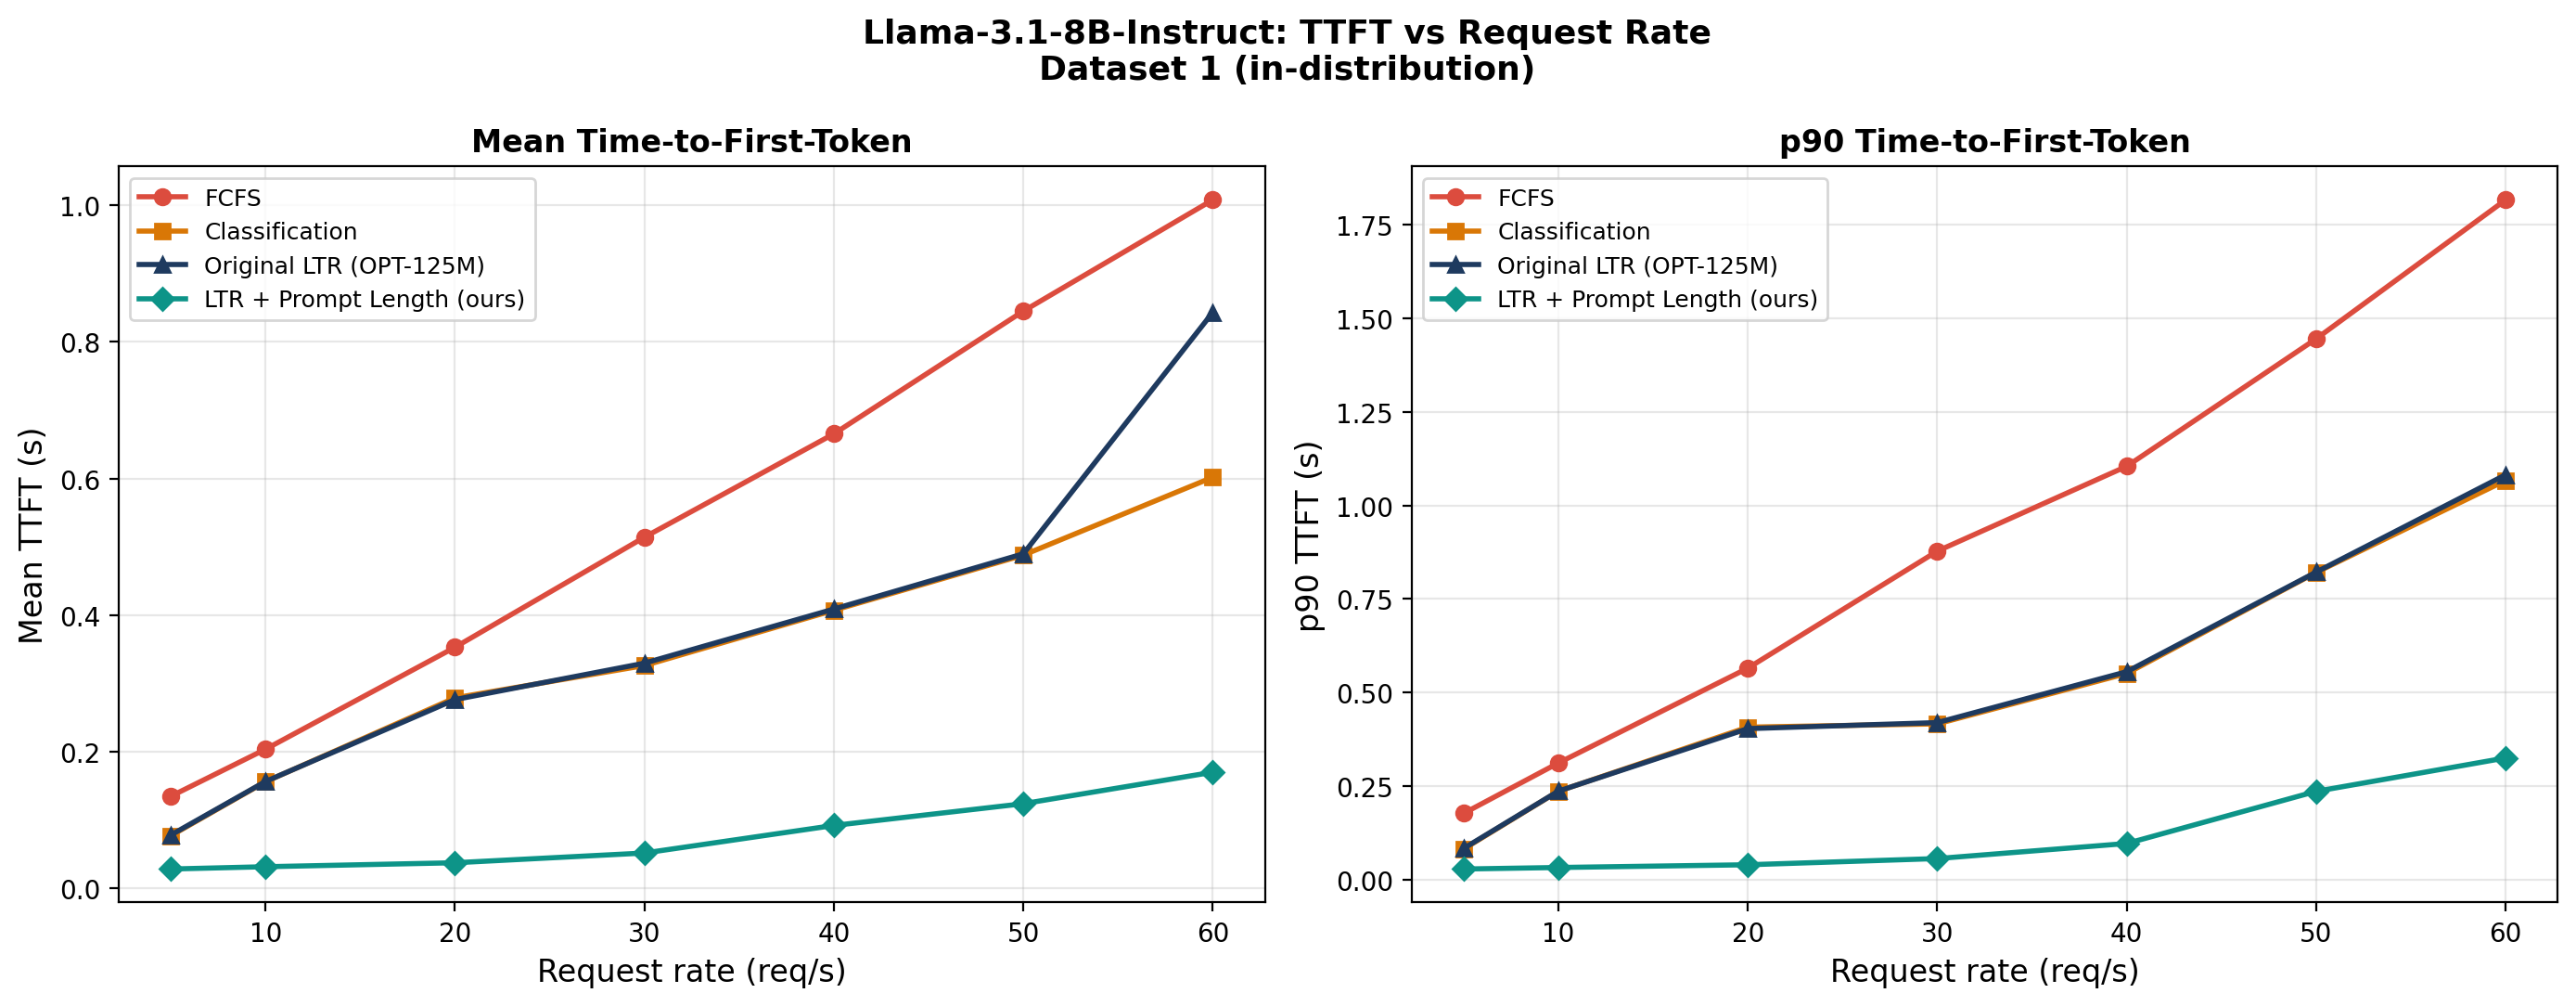
\includegraphics[width=\linewidth,height=3.5cm,keepaspectratio]{figures/ttft_dataset1.png}
        \caption{Dataset 1 (in-distribution)}
        \label{fig:ttft-d1}
    \end{subfigure}
    \hfill
    \begin{subfigure}[b]{0.48\textwidth}
        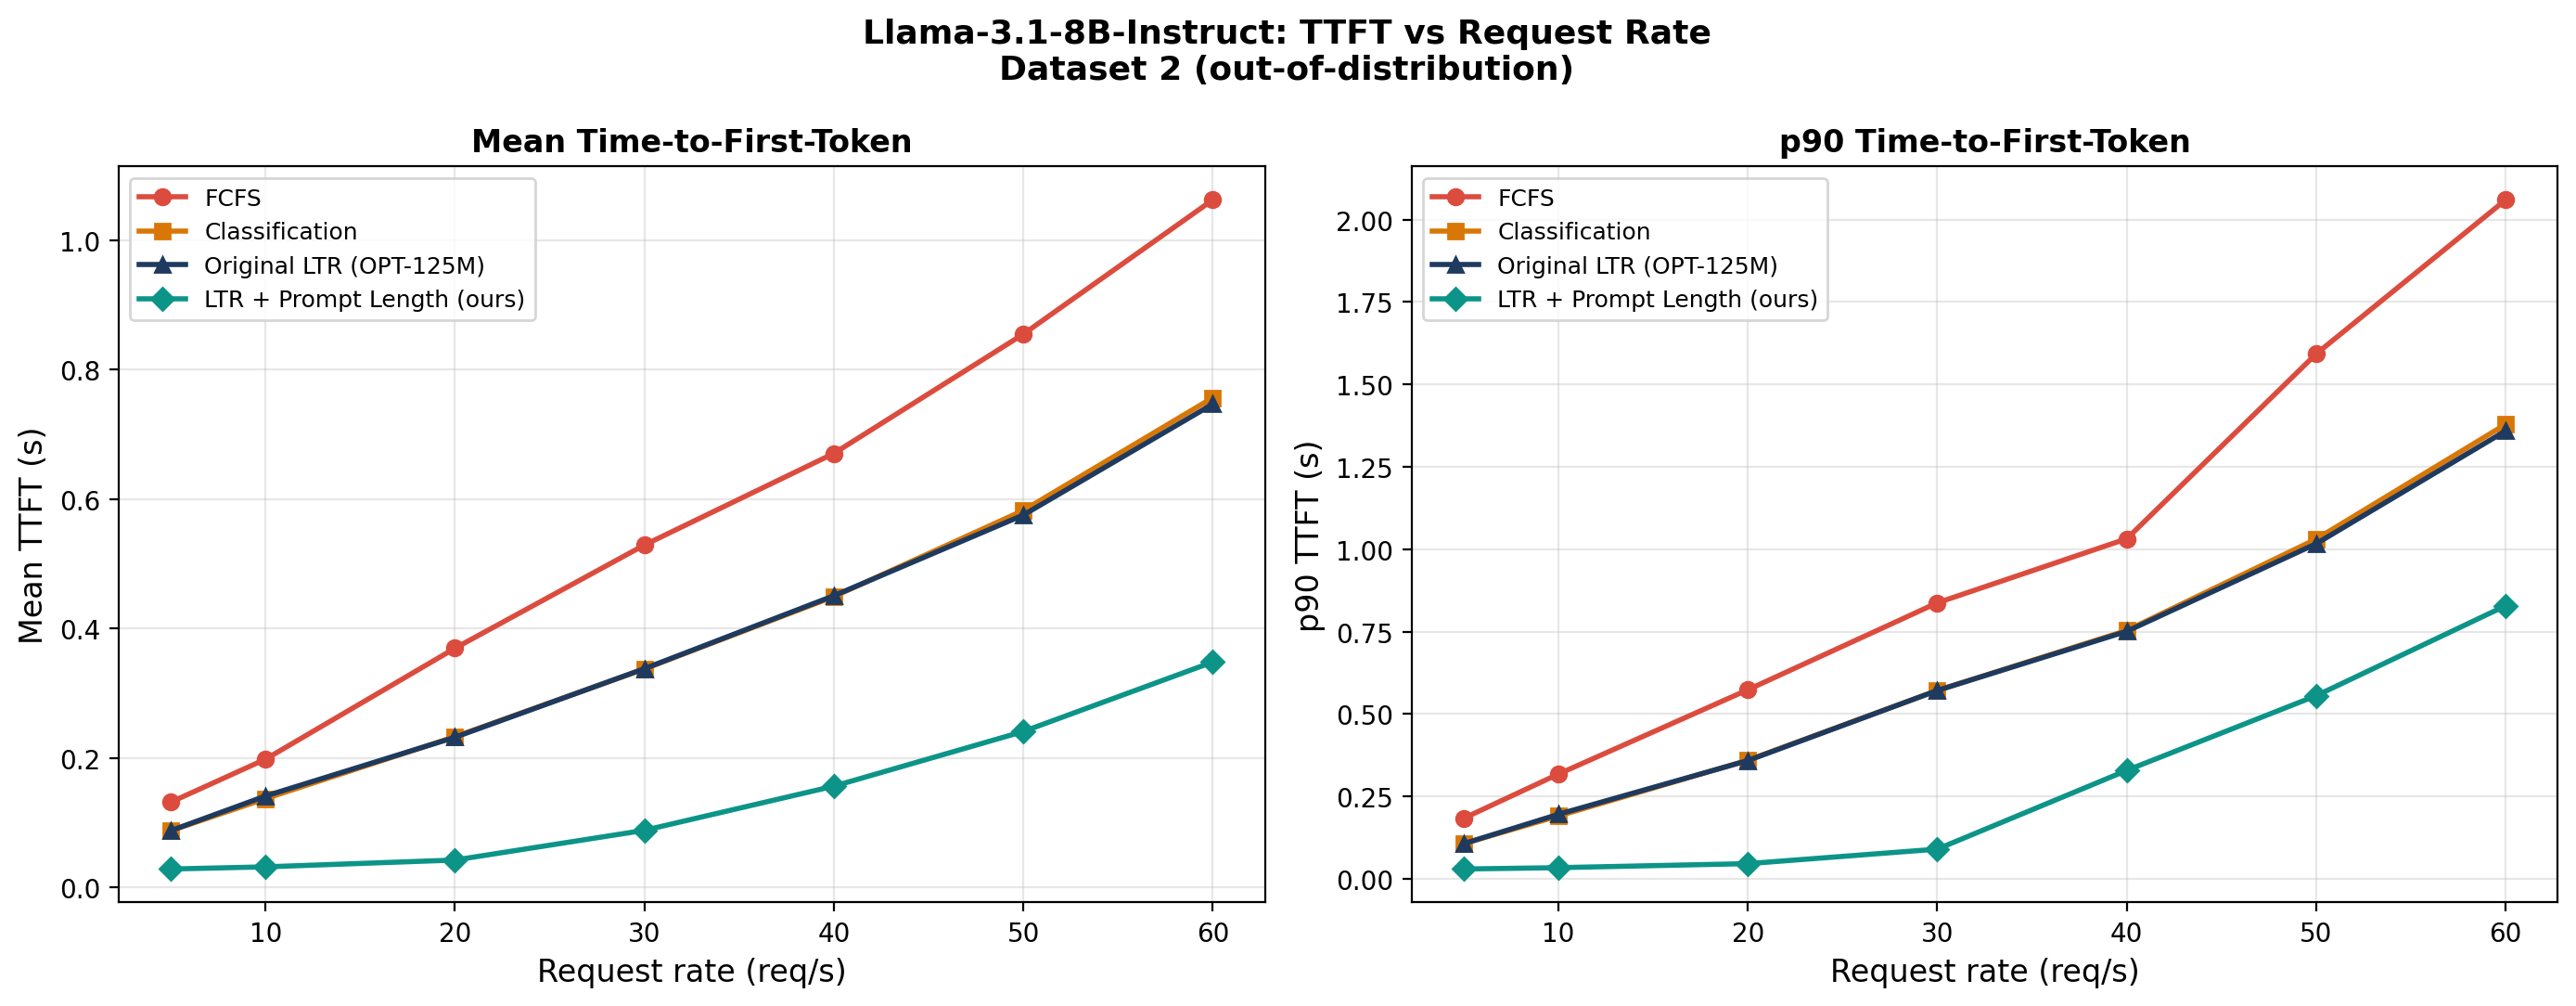
\includegraphics[width=\linewidth,height=3.5cm,keepaspectratio]{figures/ttft_dataset2.png}
        \caption{Dataset 2 (out-of-distribution)}
        \label{fig:ttft-d2}
    \end{subfigure}
    \caption{Mean and p90 time-to-first-token versus request rate, by
    scheduler.}
    \label{fig:ttft-vs-rate}
\end{figure*}

\subsection{Head-of-Line Blocking Indicators}
\label{subsec:results-hol}

Table~\ref{tab:hol_blocking} and Figure~\ref{fig:hol-blocking} summarize the
p90/mean latency ratio at high load and the latency-vs-rate slope. The
Classification and original LTR schedulers achieve the lowest p90/mean ratio
on Dataset~1, indicating that an accurate length estimate compresses tail
latency effectively; however, both show a steeper latency-vs-rate slope than
FCFS on Dataset~1, meaning latency degrades faster under load. LTR + Prompt
Length achieves the lowest slope on Dataset~2 (OOD) among all four policies,
consistent with the prompt-length signal stabilizing the ranking precisely
when the learned predictor is out of distribution.

\begin{figure*}[t]
    \centering
    \begin{subfigure}[b]{0.48\textwidth}
        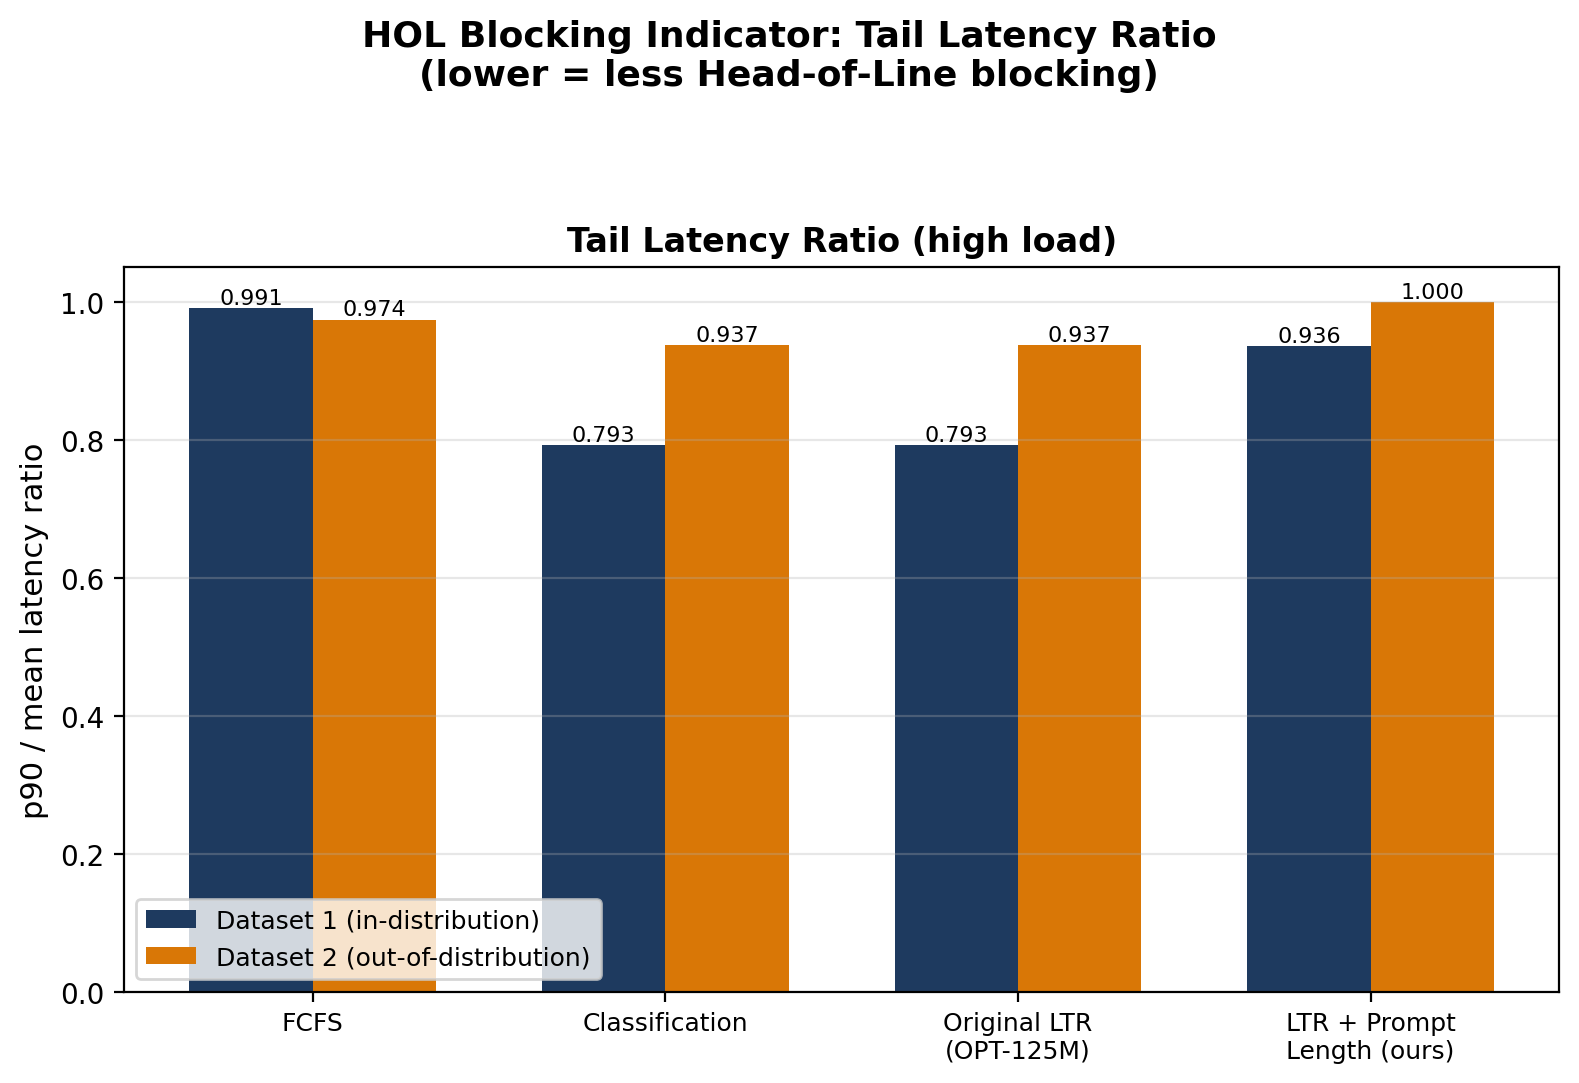
\includegraphics[width=\linewidth,height=3.5cm,keepaspectratio]{figures/hol_blocking_ratio.png}
        \caption{p90/mean latency ratio at high load}
        \label{fig:hol-ratio}
    \end{subfigure}
    \hfill
    \begin{subfigure}[b]{0.48\textwidth}
        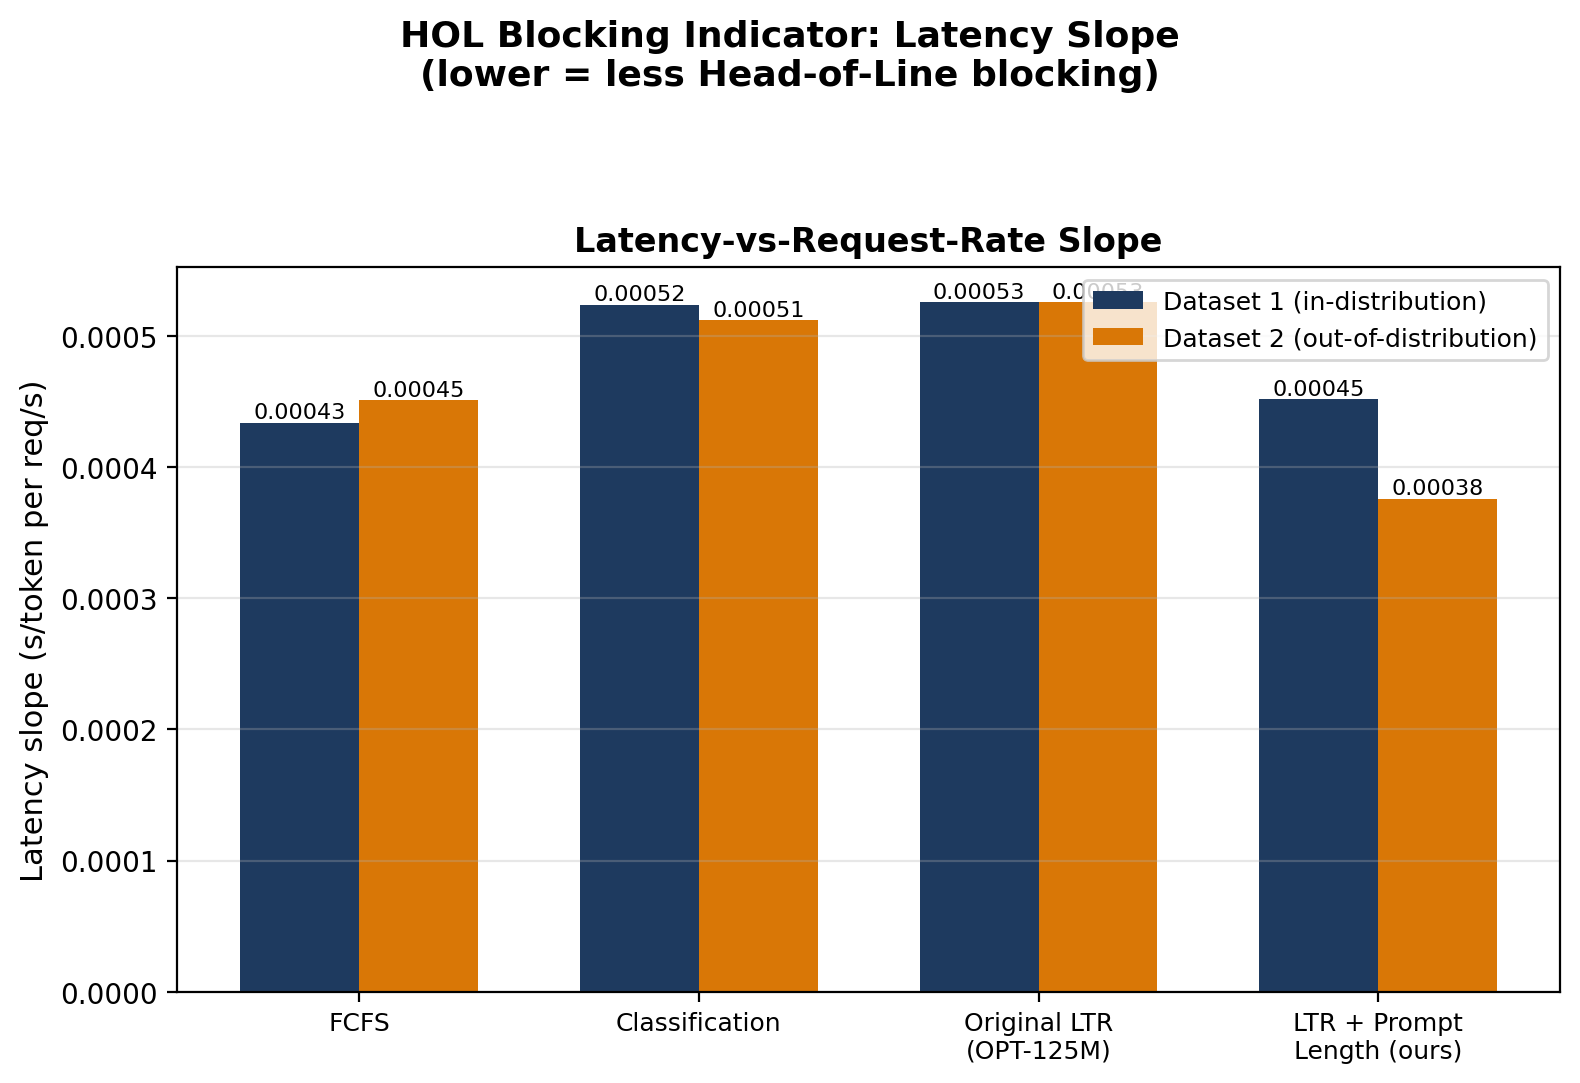
\includegraphics[width=\linewidth,height=3.5cm,keepaspectratio]{figures/hol_blocking_slope.png}
        \caption{Latency-vs-request-rate slope}
        \label{fig:hol-slope}
    \end{subfigure}
    \caption{HOL blocking indicators by scheduler and dataset.}
    \label{fig:hol-blocking}
\end{figure*}

\subsection{GPU Resource Utilization}
\label{subsec:results-gpu}

Table~\ref{tab:gpu_utilization} and Figure~\ref{fig:gpu-utilization} report
peak GPU memory allocation and utilization while serving each dataset.
Utilization stays above 86\% of the profiled budget on both datasets,
indicating the reordering step adds no meaningful memory overhead, since it
operates only on tokenized prompt lengths and predictor scores.

\begin{figure}[t]
    \centering
    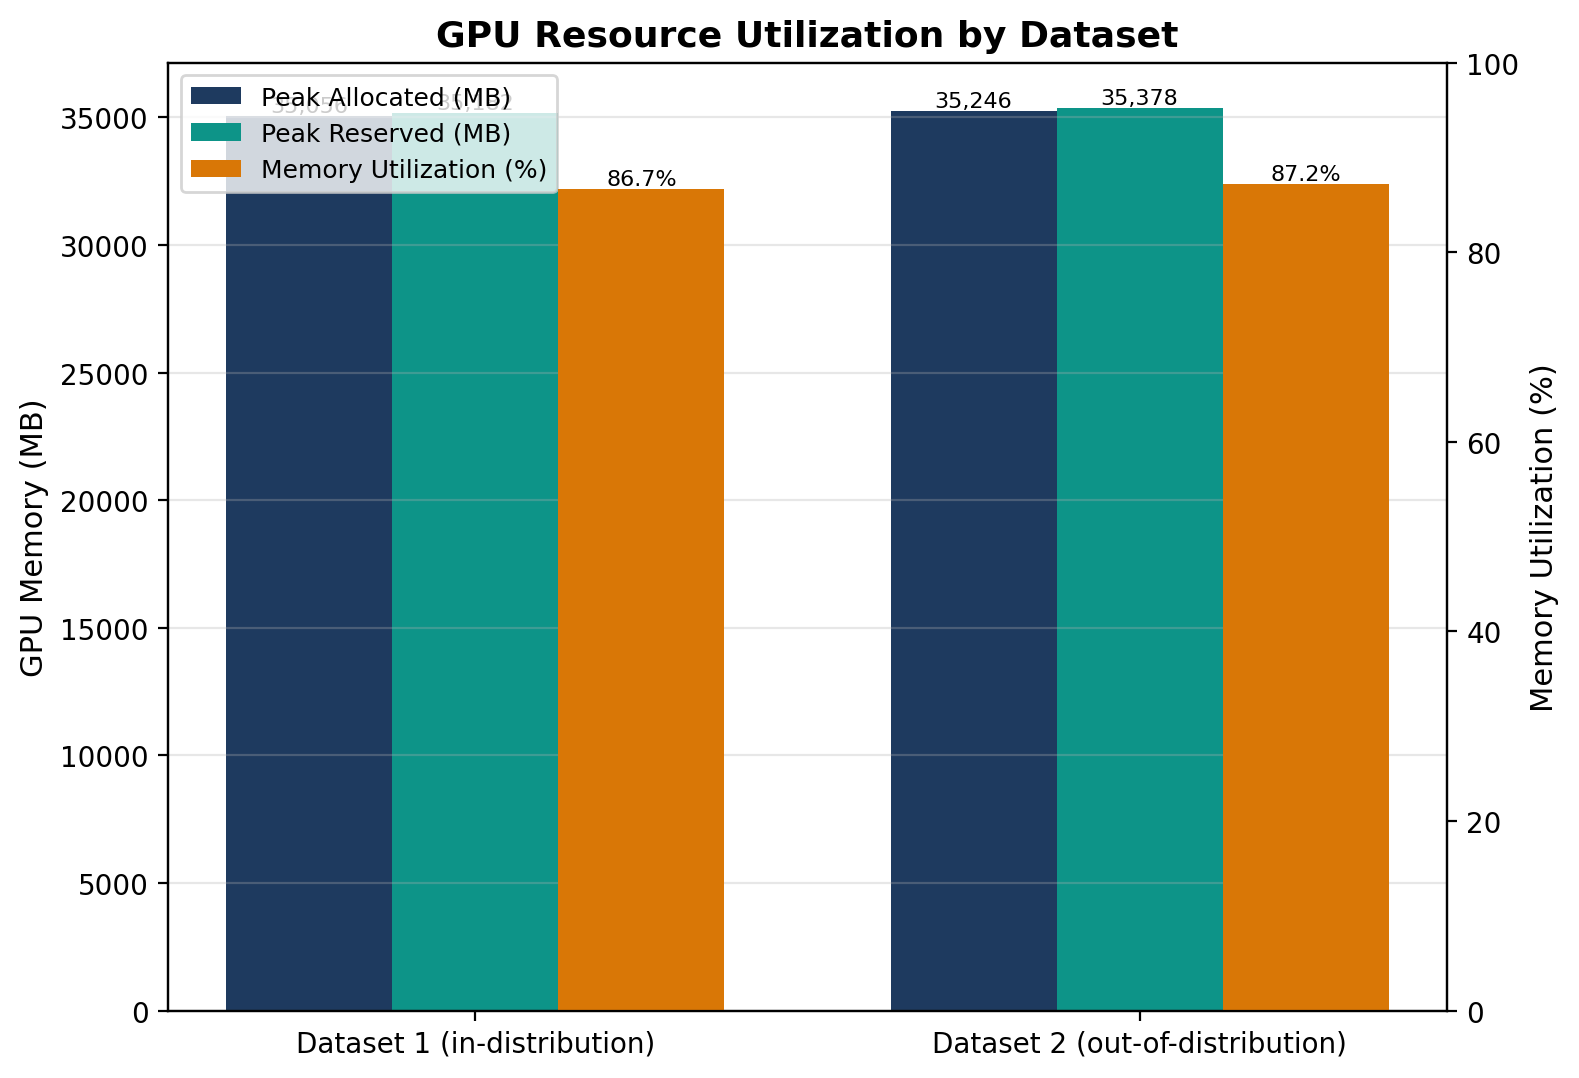
\includegraphics[width=0.8\linewidth,height=4.2cm,keepaspectratio]{figures/gpu_utilization.png}
    \caption{Peak GPU memory allocation, peak reserved memory, and memory
    utilization by dataset.}
    \label{fig:gpu-utilization}
\end{figure}

\subsection{Ranking Quality: Kendall's Tau}
\label{subsec:results-tau}

Table~\ref{tab:kendalls_tau} reports Kendall's tau between each score and
true output length on the Dataset~2 (OOD) held-out set. The composite score
modestly improves over the LTR-only score (0.3445 to 0.3457,
$\Delta=+0.0011$), indicating the prompt-length signal does not degrade
ranking quality under distribution shift.

\begin{table}[t]
    \centering
    \small
    \caption{Mean throughput (tokens/s) by scheduler.}
    \label{tab:throughput}
    \begin{tabular}{@{}lcc@{}}
        \toprule
        Scheduler & D1 (in-dist.) & D2 (OOD) \\
        \midrule
        FCFS                & 40.47 & 40.06 \\
        Classification      & 32.86 & 41.22 \\
        LTR                 & 32.80 & 41.06 \\
        LTR+PL (ours)       & \textbf{43.21} & \textbf{43.82} \\
        \bottomrule
    \end{tabular}
\end{table}

\begin{table*}[t]
    \centering
    \caption{HOL blocking indicators by scheduler: p90/mean latency ratio at
    high load (lower is better) and latency-vs-request-rate slope in
    seconds/token per req/s (lower is better).}
    \label{tab:hol_blocking}
    \begin{tabular}{@{}lcccc@{}}
        \toprule
        & \multicolumn{2}{c}{p90/mean ratio} & \multicolumn{2}{c}{Slope ($\times 10^{-4}$)} \\
        Scheduler & D1 & D2 & D1 & D2 \\
        \midrule
        FCFS                        & 0.991 & 0.974 & 4.3 & 4.7 \\
        Classification              & 0.793 & 0.937 & 5.3 & 5.2 \\
        LTR                         & 0.793 & 0.937 & 5.2 & 5.2 \\
        LTR + Prompt Length (ours)  & 0.936 & 1.000 & 4.5 & 3.8 \\
        \bottomrule
    \end{tabular}
\end{table*}

\begin{table}[t]
    \centering
    \small
    \caption{GPU resource utilization on a single NVIDIA A100 (40GB, FP16).}
    \label{tab:gpu_utilization}
    \begin{tabular}{@{}lcc@{}}
        \toprule
        Dataset & Peak alloc. (MB) & Mem. util. \\
        \midrule
        D1 (in-dist.) & 35{,}055.6 & 86.7\% \\
        D2 (OOD)      & 35{,}246.4 & 87.2\% \\
        \bottomrule
    \end{tabular}
\end{table}

\begin{table}[t]
    \centering
    \caption{Kendall's tau ranking quality against true output length,
    evaluated on the Dataset 2 (out-of-distribution) held-out set
    ($n=1{,}000$, $\alpha=0.7$, $\beta=0.3$).}
    \label{tab:kendalls_tau}
    \begin{tabular}{@{}lc@{}}
        \toprule
        Score & Kendall's $\tau$ \\
        \midrule
        LTR only                   & 0.3445 \\
        LTR + Prompt Length (ours) & 0.3457 \\
        \midrule
        $\Delta$                   & $+0.0011$ \\
        \bottomrule
    \end{tabular}
\end{table}

